%\raggedbottom
\chapter{Stato dell'arte}
In questo capitolo vengono presentate le motivazioni che hanno portato all'attivit\`a di tirocinio e le soluzioni per rilevazione di disservizi nella connettivit\`a pi\'u utilizzate.

\section{Motivazione}
Come introdotto nel precedente capitolo, lo scopo di questo tirocinio \'e di fornire una soluzione per la rilevazione di disservizi in reti locali domestiche.
Lo studio si \'e focalizzato su questo tipo di infrastrutture poich\`e esse rappresentano la maggioranza delle reti e, molto spesso, la loro configurazione \'e  lasciata ad un utente finale con poche conoscenze del campo.
Questo pu\`o portare a prestazioni poco efficienti per quanto riguarda le connessioni Wi-Fi o all'uso di apparecchiature di scarsa qualit\`a che dimuiscono le velocit\`a di download ed upload dei dispositivi.
In aggiunta, access point vicini, se sullo stesso canale Wi-Fi,potrebbero interferire sulla connessione locale.
Per questo motivo, software come Kismet\cite{kismet}, possono essere utilizzati anche per scegliere un canale non sovrautilizzato oltre a monitorare il traffico Wi-Fi ed i device connessi ad una rete.
Negli ultimi tempi, i produttori di router, stanno cercando di implementare in tutti i loro dispositivi metodi di monitoraggio per rilevare disservizi di reti.
Questo permette agli Internet Service Providers (ISP) di fornire una diagnostica iniziale che circoscriva il problema all'interno o all'esterno della rete.
Nel primo caso, l'utente viene informato della presenza del problema nella sua rete locale e quali dispositivi ne siano affetti, mentre nel secondo caso \'e il fornitore del servizio Internet a dover intervenire sulla propria rete per rimediare al disservizio.
Le soluzioni attuali per il monitoraggio e la gestione di rete presentano infatti diverse problematiche quando applicate a reti piccole locali.
\newpage
In particolare il software \'e:
\begin{itemize}
	\item Ristretto ad apparecchiature di fascia alta.
	\item Non sempre fornito di interoperabilit\`a con software di altri produttori.
	\item Difficile da utilizzare per personale non specializzato.
\end{itemize}

Per questi motivi l'elaborato vuol fornire, dopo aver introdotto le tecniche di rilevazione di disservizi pi\`u comuni, una soluzione che possa essere utilizzata in piccole reti da utenti non esperti e su apparecchiature non professionali.

\section[IEEE 802.11 Distributed Coordination Function]{IEEE 802.11 \\Distributed Coordination Function}
Nel protocollo 802.11 il meccanismo di accesso al mezzo trasmissivo \'e chiamato distributed coordination function (DCF) \cite{ieee99}.
Questo metodo di accesso casuale \'e basato sul protocollo di accesso multiplo tramite rilevamento della portante con evitamento delle collisioni (CSMA/CA) in cui i terminali tentano di evitare a priori il verificarsi di collisioni durante la trasmissione.
La ritrasmissione, in caso di collisione di pacchetti, \'e gestita tramite un algoritmo di backoff esponenziale binario (BEB) che verr\`a presentato in dettaglio successivamente.
\'E importante notare che lo standard IEEE 802.11 definisce anche un  protocollo opzionale, chiamato point coordination function (PCF), in cui l'access point ha il compito di coordinare l'accesso al mezzo trasmissivo per evitare collisioni. 
Questo tipo di meccanismo di accesso non verr\`a trattato per via del suo poco utilizzo.

DCF descrive due tecniche per la trasmissione di pacchetti:
\begin{itemize}
 \item Two-way handshake: meccanismo di accesso base.
 \item Four-way handshake: request to send/clear to send (RTS/CTS).
\end{itemize}

Il meccanismo di accesso base \'e ottenuto attraverso la trasmissione immediata di un acknowledgment positivo (ACK) da parte della stazione destinataria dopo aver ricevuto correttamente un pacchetto dal mittente.
L'invio esplicito dell'ACK \'e richiesto poich\`e in un mezzo trasmissivo senza fili il mittente non pu\`o determinare se il pacchetto sia stato ricevuto correttamente ascoltando la sua stessa trasmissione.

Il meccanismo RTS/CTS \'e opzionale e prevede che una stazione interessata all'invio di un pacchetto riservi il mezzo trasmissivo tramite un pacchetto request to send.
Dopo che il destinatario riconosce questo pacchetto con un frame CTS la comunicazione continua con l'invio del pacchetto desiderato e di relativo ACK.

Questo meccanismo permette l'incremento della performance del sistema grazie alla riduzione della durata di collisione che potrebbe avvenire con l'invio di lunghi pacchetti.
Infatti, in questo caso, la collisione pu\`o solamente avvenire sul frame RTS e viene riconosciuta dalla mancanza di un frame CTS di risposta del destinatario.
In aggiunta il meccanismo RTS/CTS implementato nello standard IEEE 802.11 \'e sviluppato per contrastare il problema dei terminali nascosti \cite{tobagi1975packet} che si presenta quando un paio di stazioni mobili non riescono a rilevarsi. %Migliorare questa parte, aggiungere reference

Si presenta ora il funzionamento di DCF, come standardizzato dal protocollo 802.11.

Una stazione che vuole trasmettere un pacchetto, prima di inviarlo, monitora l'attivit\`a presente sul canale.
Se il canale risulta inattivo per una durata pari ad un distributed interframe space (DIFS), il mittente procede all'invio del frame.
In caso contrario, se il canale \'e attualmente in uso, la stazione continua a monitorarlo finch\`e esso non risulta inattivo per un DIFS.
A questo punto la stazione attende per un intervallo casuale di backoff per minimizzare la probabilit\`a di collisione di pacchetti con altre stazioni che hanno intenzione di trasmettere.
Nello stesso modo, una stazione dovr\`a attendere un altro intervallo casuale per l'invio di due pacchetti consecutivi, anche se il canale risulta inattivo per un DIFS in modo da non impossessarsi del canale di trasmissione.
L'uso del backoff casuale \'e il meccanismo che questo protocollo implementa per la collision avoidance.

DCF utilizza una scala a tempo discreto di backoff per motivi di efficienza, infatti il tempo immediatamente successivo ad un DIFS viene diviso in slot ed ogni stazione pu\`o solo trasmettere all'inizio di ciascuno di questi.
\begin{wraptable}{r}{6cm}
%\begin{flushright}
\centering
\begin{tabular}{| l | l | l | l |}
	\hline 
	PHY & $\delta$ & CW\textsubscript{min} & CW\textsubscript{max} \\ \hline
	FHSS & 50 & 16 & 1024 \\ \hline
	DSSS & 20 & 32 & 1024 \\ \hline
	IR &8 & 64 & 1024 \\ 
	\hline
\end{tabular}
%\end{flushright}
\caption{Valori $\delta$}
\label{table:deltavalues}
\end{wraptable}

La dimensione dello slot, $\delta$,  \'e pari al tempo che una stazione impiega per rilevare la trasmissione di un pacchetto da parte di una qualsiasi altra stazione.
Questo valore dipende dal tipo dal tipo del mezzo trasmissivo e viene raffigurato nella tabella \ref{table:deltavalues}.
Come precedentemente introdotto, DCF, implementa un backoff esponenziale ed il tempo viene scelto in un range (0, $\omega$-1) dove $\omega$ \'e detta contention window.
Questo valore dipende dal numero di trasmissioni fallite per un pacchetto, a partire da un valore pari a CW\textsubscript{min}  viene raddoppiata ad ogni trasmissione fallita fino ad un valore massimo pari a CW\textsubscript{max}=2\textsuperscript{m} CW\textsubscript{min}.
I valori minimi e massimi della finestra sono specificati, a seconda del tipo di mezzo di trasmissione, nella tabella \ref{table:deltavalues}.
Il contatore del backoff viene decrementato quando il canale si trova in uno stato di idle mentre \'e mantenuto inalterato quando una trasmissione viene captata sul canale.
Infine, la stazione trasmette quando il valore del contatore raggiunge lo 0.

Si presentano ora due esempi di trasmissione usando i due metodi di accesso al metodo trasmissivo presentati.

Considerando due stazioni A e B che condividono lo stesso canale utilizzando il metodo base di accesso, alla fine della trasmissione B attende un DIFS e sceglie un tempo di backoff prima di trasmettere un nuovo pacchetto.
Durante questo periodo la stazione A invia un pacchetto sul canale e, di conseguenza, il timer di backoff della stazione B rimane invariato fino a che il canale non verr\`a percepito come libero per almeno un DIFS.
Per quanto riguarda la stazione A, essa riceve un ACK per segnalare la ricezione con successo del pacchetto da parte del destinatario.
Il pacchetto di ACK viene inviato immediatamente trasmesso alla fine del messaggio, dopo un periodo di attesa chiamato short interframe space (SIFS).
La durata di un SIFS \'e inferiore a quella di un DIFS, questo rende impossibile alle altre stazioni di rilevare come libero il canale fino a che non venga inviato l'ACK.
In caso di mancata ricezione dell'ACK da parte della stazione A entro un tempo specificato ACKTimeout o della trasmissione di altri pacchetti nel canale, questa rischedula l'invio del pacchetto tramite le regole di backoff presentate.

Nel meccanismo RTS/CTS una stazione che vuole trasmettere un pacchetto aspetta fino a che non rileva il canale inattivo per un DIFS, segue le regole di backoff precedentemente introdotte e trasmette un frame speciale chiamato RTS.
Quando la stazione ricevente riconosce un frame RTS risponde, dopo un SIFS di attesa, con un frame CTS.
Il mittente \'e autorizzato ad utilizzare il canale solo alla corretta ricezione di un CTS.
I frame RTS e CTS contengono inoltre la lunghezza del pacchetto da trasmettere, permettendo a tutte le stazioni in ascolto di aggiornare un network allocation vector (NAV) contenente il periodo di tempo per il quale il canale sar\`a occupato.
Questo meccanismo fornisce, quindi, una soluzione al problema dei terminali nascosti oltre a ridurre la lunghezza dei frame coinvolti nella contesa del canale.

%\vspace{5mm}
\begin{figure}[!htb]
	\centering
	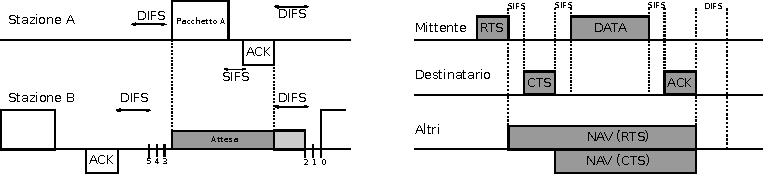
\includegraphics{images/img1.pdf}
	\caption{DCF con metodo accesso base (sinistra) e RTS/CTS (destra)}
	\label{fig:dcfex}
\end{figure}

%\section{Performance analysis of the IEEE 802.11 distributed coordination function}
\section{Analisi della performance IEEE 802.11 DCF}
Uno dei primi e pi\`u rilevanti studi sulle prestazioni del meccanismo DCF \'e quello svolto da Bianchi \cite{bianchi2000performance} che propone la valutazione analitica del saturation throughput, ovvero il limite del throughput di sistema raggiunto all'aumentare del carico sul sistema stesso.
L'analisi \'e stata effettuata con un numero fissato di stazioni ed uno stato di saturazione, ovvero assumendo che ogni stazione abbia sempre un pacchetto disponibile ad essere trasmesso.
Diviso in due parti, lo studio improntato da Bianchi si concentra prima nel fornire una rappresentazione in catena di Markov del comportamento della singola stazione per ottenere la probabilit\`a stazionaria $\tau$ che essa trasmetta un pacchetto in uno slot di tempo casuale.
L'approccio utilizzato fornisce una probabilit\`a indipendente dal tipo di meccanismo di accesso (base o RTS/CTS).
Dopo aver trovato questo valore, analizzando i possibili eventi che possono accadere in un determinato slot temporale, lo studio si conclude esprimendo il throughput dei due possibili metodi di accesso al mezzo trasmissivo in funzione del valore $\tau$.

$$
\begin{cases}
  P \{ i, k| i, k + 1\}  =1 	 &\qquad k \in (0, W_{i}-2) \ i \in (0,m) \\ 
  P \{ 0, k| i, 0\}  =(1-p)/W_{0} 	 &\qquad k \in (0, W_{0}-1) \ i \in (0,m) \\ 
  P \{ i, k| i-1, 0\}  =p/W_{i} 	 &\qquad k \in (0, W_{i}-1) \ i \in (1,m) \\ 
  P \{ m, k| m, 0\}  =p/W_{m} 	 &\qquad k \in (0, W_{m}-1) \\
\end{cases}
$$

La prima equazione tiene conto del decremento del tempo di backoff all'inizio di ogni slot di tempo mentre la seconda equazione del fatto che un nuovo pacchetto in seguito ad una trasmissione con successo inizia con un backoff stage pari a 0.
I restanti due casi esprimono il sistema in caso di fallimento nella trasmissione.
In particolare la terza equazione esprime come avvenga un aumento del backoff stage e la scelta di un nuovo valore di backoff iniziale nel range (0,W\textsubscript{i}).
Infine, l'ultima equazione, modella il massimo valore m che il tempo di backoff pu\`o assumere.
Dopo aver trovato la formula chiusa della catena di Markov si pu\`o esprimere la probabilit\`a $\tau$ che una stazione trasmetta in uno slot di tempo casuale.
Poich\`e la trasmissione avviene quando il timer di backoff raggiunge lo 0, a prescindere dal backoff stage il valore di $\tau$ \'e pari a:


\begin{equation}
\tau = \frac{2(1-2p)}{(1-2p)(W+1)+pW(1-(2p)^m)}
\end{equation}

Il valore di p, ovvero della probabilit\`a di collisione, \'e pari alla probabilit\`a che una delle restanti n-1 stazioni decida di trasmettere un pacchetto.

\begin{equation}
p =1-(1-\tau)^{n-1}
\end{equation}

Possiamo quindi dire che 

\begin{equation}
\tau(p) = \frac{2}{1+W+pW \sum_{i=0}^{m-1}(2p)^i}
\end{equation}

Per calcolare quindi S, il throughput normalizzato, ovvero il periodo di tempo in cui il canale \'e utilizzato per trasmettere correttamente pacchetti, Bianchi ha poi definito le probabilit\`a degli eventi che possono accadere in uno slot di tempo.
In particolare, viene identificata con P\textsubscript{tr} la probabilit\`a che ci sia almeno una trasmissione nello slot di tempo e, poich\`e ogni stazione trasmette sul canale con probabilit\`a $\tau$, si ha:

\begin{equation}
P_{tr} = 1-(1-\tau)^n
\end{equation}

La probabilit\`a P\textsubscript{s} che una trasmissione avvenga correttamente \'e quindi data dalla probabilit\`a che esattamente una stazione trasmetta condizionata dalla probabilit\`a che almeno una stazione trasmetta.

\begin{equation}
P_{s} = \frac{n\tau(1-\tau)^{n-1}}{P_{tr}} = \frac{n\tau(1-\tau)^{n-1}}{ 1-(1-\tau)^n}
\end{equation} 

Si pu\`o ora descrivere S come il rapporto

\begin{equation}
S = \frac{E[payload \ trasmesso \ in \ uno \ slot \ di \ tempo]}{E[lunghezza \ dello \ slot \ di \ tempo]}
\end{equation}

Dato che E[P] e' la dimensione media di un pacchetto, la media di informazione trasmessa correttamente in uno slot di tempo e' pari a $P_{tr}P_{s}E[P]$, poich\`e una trasmissione corretta avviene in uno slot con probabilit\`a $P_{tr}P_{s}$.
Con probabilit\`a $1-P_{tr}$ lo slot di tempo \'e vuoto, con probabilit\`a $P_{tr}P{s}$ contiene una trasmissione con successo e con probabilit\`a $P_{tr}(1-P_{s})$ una collisione.
L'equazione per ottenere S diventa quindi
\begin{equation}
S = \frac{P_{s} P_{tr} E[P]}{	(1-P_{tr})\sigma + P_{tr} P\textsubscript{s} T_{s} + P_{tr}(1-P_{s})T_{c}}
\end{equation}

In questa equazione si identifica il tempo medio in cui il canale viene visto come occupato per via di una trasmissione avvenuta con successo con $T_{s}$ ed il tempo medio in cui il canale viene visto come occupato per via di una trasmissione con collisione con $T_{c}$.
Questi valori, necessari per il calcolo del throughput, dipendono dal tipo di meccanismo di accesso utilizzato.
Per quanto riguarda il meccanismo di accesso base, identificando con H=$ PHY_{hdr}$ + $MAC_{hdr}$, $\delta$ il ritardo di propagazione e E[P*] la lunghezza media del pi\`u grande pacchetto coinvolto in una collisione:

$$
\begin{cases}
T_{s}^{bas} &= H + E[P] + SIFS + \delta + ACK + DIFS + \delta \\
T_{c}^{bas} &= H + E[P*] + DIFS + \delta \\
\end{cases}
$$

Per il meccanismo di accesso basato su RTS/CTS i valori sono invece

$$
\begin{cases}
\!\begin{aligned}
T_{s}^{rts} =  &\ RTS + SIFS + \delta + CTS + SIFS + \delta + H + E[P]  \\ & + SIFS + \delta + ACK + DIFS + \delta 
\end{aligned}
\\
T_{c}^{rts} = RTS + DIFS + \delta \\
\end{cases}
$$

Il modello presentato da Bianchi si \'e rivelato, dopo validazione tramite simulazione, efficace per rappresentare i diversi schemi di accesso utilizzati da DCF: in particolare quello base, RTS/CTS ed una combinazione dei due che non \'e stata riportata.
I risultati ottenuti dal modello mostrano che la performance del metodo di accesso base dipende fortemente sui parametri del sistema, principalmente il numero di stazioni connessi ed i parametri minimi della finestra di contesa.
Questi ultimi sono per\`o meno influenti sul metodo RTS/CTS che si presenta come la migliore opzione di accesso al mezzo trasmissivo per reti di grandi dimensioni per via della possibilit\`a di arginare il problema dei terminali nascosti ed un minore tempo impiegato durante la collisione quando pi\`u stazioni trasmettono contemporaneamente.

\newpage

\section{TCP e DCF, analisi della performance }

Lo studio condotto da Wu et al \cite{wu2002performance} propone un modello basato su quello di Bianchi che tiene per\`o conto del limite di tentativi di ritrasmissione di un frame.
In aggiunta, viene proposto un miglioramento allo standard 802.11 con l'introduzione di DCF+.
Questo meccanismo di accesso al metodo di trasmissione \'e introdotto per cercare di sopperire alle problematiche di performance di cui protocolli di livello trasporto soffrono in reti wireless \cite{xylomenos1999tcp}.
In particolare, lo studio si concentra sul risolvere la contesa per il canale di trasmissione che avviene durante lo scambio di dati ed ACK TCP, meccanismo che potrebbe causare collisioni ed un degrado delle prestazioni.
La soluzione proposta \'e inoltre compatibile con DCF definito dallo standard 802.11, questo vuol dire che in una stessa rete possono coesistere e comunicare stazioni che supportano due metodi di accesso al mezzo trasmissivo diversi.

Il principale cambiamento che DCF+ apporta \'e quello di utilizzare il MAC ACK specificato nello standard 802.11 come un RTS.
Questo \'e in linea con l'implementazione di DCF che prevede l'invio di un ACK in caso di una trasmissione ricevuta con successo e permette una retrocompatibilit\`a con stazioni che non implementano DCF+.

In figura \ref{fig:dcf+ex} si mostra un esempio del funzionamento di DCF+ assumendo che la stazione destinatario debba, oltre a ricevere un frame dal mittente, anche inviargli un pacchetto dati.
Successivamente alla corretta ricezione del frame dati il destinatario procede ad inviare un ACK al mittente che, come gi\`a introdotto, viene considerato come un RTS ed utilizzato per inizializzare anche il NAV delle altre stazioni in ascolto. 
Come da implementazione del DCF il mittente risponde a questo frame con un CTS ed inizializza i valori del NAV pari alla lunghezza del frame di dati che deve ricevere.
L'operazione si conclude con l'invio del pacchetto ed un normale ACK di riscontro.
Per quanto riguarda il metodo di accesso RTS/CTS la procedura differisce solo per l'aggiunta dei due pacchetti iniziali che permettono alle stazioni di impossessarsi del mezzo trasmissivo.

\begin{figure}[!htb]
	\centering
	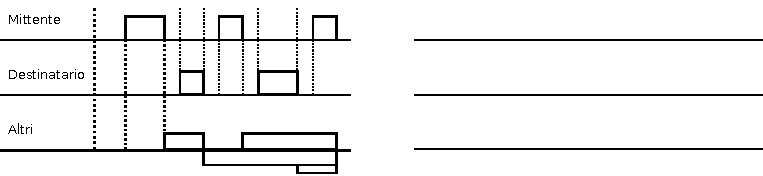
\includegraphics{images/img2.pdf}
	\caption{DCF+ con metodo accesso base (sinistra) e RTS/CTS (destra)}
	\label{fig:dcf+ex}
\end{figure}

Il funzionamento di DCF+ come presentato si basa, per\`o, su due assunzioni:

\begin{itemize}
	\item La stazione mittente che riceve l'ACK sia in grado di determinare, in base al campo della durata presente nel frame, se il destinatario ha un pacchetto dati pronto per l'invio.
	\item Le stazioni, tramite campi nel frame dati e record locali, siano in 		grado di determinare se il destinatario supporti DCF+.
\end{itemize}

Il modello utilizzato da Wu et al per l'analisi di questo metodo di accesso si basa su una estensione del modello proposto da Bianchi.
In particolare, a parit\`a di assunzioni, viene proposta una catena di Markov in cui vengono considerati gli effetti del limite di ritrasmissioni di frame:

$$
\begin{cases}
  P \{ i, k| i, k + 1\}  =1 	 &\qquad k \in (0, W_{i}-2) \ i \in (0,m) \\ 
  P \{ 0, k| i, 0\}  =(1-p)/W_{0} 	 &\qquad k \in (0, W_{0}-1) \ i \in (0,m) \\ 
  P \{ i, k| i-1, 0\}  =p/W_{i} 	 &\qquad k \in (0, W_{i}-1) \ i \in (1,m) \\ 
  P \{ 0, k| m, 0\}  =p/W_{0} 	 &\qquad k \in (0, W_{m}-1) \\
\end{cases}
$$

%b0,0

Questa differenza si ripercuote anche sui valori di $\tau$ e $p$.
In aggiunta, poich\`e viene considerato anche l'effetto timeout dell'ACK, il modello differir\`a da quello proposto da Bianchi anche nei valori di $T^{bas}$ e $T^{rts}$ che saranno, rispettivamente:

$$
\begin{cases}
T_{s}^{bas} &= H + E[P] + SIFS + \delta + ACK + DIFS + \delta \\
T_{c}^{bas} &= DIFS + H + E[P*] + SIFS + ACK \\
\end{cases}
$$

$$
\begin{cases}
\!\begin{aligned}
T_{s}^{rts} =  &\ RTS + SIFS + \delta + CTS + SIFS + \delta + H + E[P]  \\ & + SIFS + \delta + ACK + DIFS + \delta 
\end{aligned}
\\
T_{c}^{rts} = DIFS + RTS + SIFS + CTS \\
\end{cases}
$$

Il modello analitico sviluppato da questo studio si \'e dimostrato pi\`u accurato rispetto a quello proposto da \cite{bianchi2000performance} in seguito alle simulazioni svolte.
Quest'ultimo infatti sovrastima il throughput poich\`e non considera il limite di ritrasmissioni ed il timeout dovuto all'ACK.
Le prestazioni di DCF+ sono poi state comparate a quelle di DCF utilizzando il modello presentato, evidenziando un miglioramento in metriche quali: goodput, fairness nell'utilizzo del mezzo trasmissivo e delay a livello MAC.

\newpage
\section{IEEE 802.11E EDCF}
Fino allo standard IEEE 802.11e \cite{ieee05} il modello della WLAN pu\`o essere visto come una versione wireless di Ethernet che supporta un servizio best effort.
L'aumento dei servizi offerti in streaming e VoIP ha per\`o reso necessaria l'implementazione di meccanismi per il supporto quality of service (QoS), ovvero la possibilit\`a di fornire una diversa priorit\`a a diverse applicazioni o utenti.
Nel principio 802.11 non fornisce questo supporto di differenziare frame in base a priorit\`a, tutto ci\`o che fornisce DCF \'e un accesso al canale in contesa con uguale probabilit\`a per tutte le stazioni.
Lo standard 802.11e definisce due miglioramenti al fine di supportare QoS mediamente l'introduzione di Enhanced Distributed Coordination Function (EDCF) e Hybrid Coordination Function (HCF).
In EDCF vengono implementate delle categorie di traffico (TC) a cui vengono associate diverse priorit\`a come mostrato nella tabella \ref{table:catvalues}.

%\begin{flushright}
\begin{table}[h]
%\centering
\begin{tabular}{| l | l | l | l |}
	\hline 
	Priorit\`a  & 802.1D & Categoria & Descrizione \\ \hline
	Bassa & 1 & AC\textunderscore BK & Background \\ \hline
     & 2 & AC\textunderscore BK & Background \\ \hline
	 & 0 & AC\textunderscore BE & Best Effort \\ \hline
	 & 3 & AC\textunderscore BK & Best Effort \\ \hline
	 & 4 & AC\textunderscore VI & Video \\ \hline
	 & 5 & AC\textunderscore VI & Video \\ \hline
	 & 6 & AC\textunderscore VO & Voce \\ \hline
	Alta & 7 & AC\textunderscore VO & Voce \\ \hline
\end{tabular}
%\end{flushright}
\centering
\caption{Tabella categorie accesso}
\label{table:catvalues}
\end{table}

I frame delle stazioni vengono quindi divisi in diverse istanze di backoff, ognuna con dei parametri specifici alla categoria di traffico \ref{fig:edcf}.
Nel periodo di contesa per il mezzo trasmissivo, ogni categoria di traffico cerca di accedere ad una transmission opportunity (TXOP) ed inizia un periodo di backoff indipendente dopo che il canale \'e inattivo per almeno un Arbitration Interframe Space (AIFS).
Se durante il periodo di backoff il canale torna ad essere utilizzato, come per DCF, EDCF aspetta che il canale torni ad essere libero prima di diminuire il valore di backoff.
Per via delle categorie di traffico, una singola stazione pu\`o implementare fino ad otto code interne realizzate come stazioni virtuali.
Se pi\`u di una stazione raggiunge il valore 0 nel backoff, uno scheduler ha il compito di evitare una collisione tra le due stazioni virtuali dando la TXOP alla stazione con priorit\`a pi\`u alta.

\begin{figure}[!htb]
	\centering
	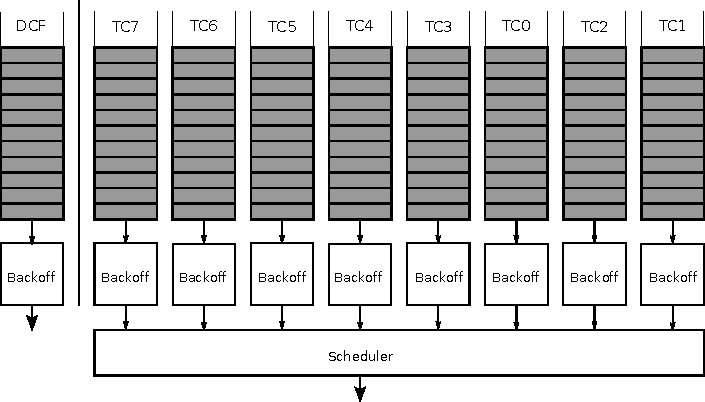
\includegraphics{images/img3.pdf}
	\caption{DCF (sinistra) e EDCF con otto backoff virtuali (destra)}
	\label{fig:edcf}
\end{figure}

Durante l'intervallo TXOP, definito da un tempo di inizio ed una massima durata, una stazione ha il diritto di trasmettere sul canale.
L'intervallo TXOP viene allocato tramite una contesa (EDCF-TXOP) o assegnato attraverso HCF (polled-TXOP).
La durata dell'intervallo \'e definita dai beacon frames dell'AP per quanto riguarda EDCF-TXOP e specificato nel frame del poll per quanto riguarda HCF.

Diversi studi sono stati improntati sulla performance di EDCF, in particolare \cite{mangold2002ieee} dopo aver simulato l'uso di EDCF ne evidenzia una soluzione efficiente per l'implementazione QoS su reti WLAN e la retrocompatibilit\`a con stazioni che non implementano questo metodo di accesso.
Con l'opportuna scelta di parametri, stazioni EDCF riescono infatti ad avere priorit\`a sul canale rispetto a stazioni che implementano DCF.

Xiao \cite{xiao2004performance} ha successivamente fornito un modello analitico, seguendo le orme di Bianchi, di EDCF.
Utilizzando metriche di backoff quali: dimensione iniziale della finestra, limite di ritrasmissioni e il fattore di incremento della finestra di backoff i risultati ottenuti dallo studio mostrano come una categoria di traffico possa rubare banda ad un'altra categoria in caso questa aumenti il valore delle suddette metriche.
In aggiunta, viene suggerita una ridimensione del limite di ritrasmissioni per traffico di tipo video per aumentare throughput e migliorare il delay.

\newpage


\section{IEEE 802.11N e 802.11AC}

Attualmente la maggior parte dei router in commercio ed utilizzati in reti locali sono conformi allo standard 802.11n ed, in particolare, a quello 802.11ac.
Il primo, con l'obiettivo di aumentare il throughput degli standard precedenti, fornisce supporto per frame aggregation e multiple-input and multiple-output (MIMO).
Come suggerisce il nome, il frame aggregation permette ad un trasmettitore di inviare pi\`u di un frame in una singola trasmissione.
Questa funzionalita, come studiato da  \cite{skordoulis2008ieee}, si rivela molto efficace per l'aumento del throughput della rete e per la riduzione del ritardo di trasmissione.
La tecnologia MIMO fa utilizzo di una moltitudine di antenne in ricezione ed invio per trasmettere simultaneamente pi\`u stream di dati utilizzando propagazione a pi\`u vie.
Il successivo standard 802.11ac, utilizzato maggiormente nella realizzazione del tirocinio, estende MIMO per permettere un uso multi utente, chiamato  MU-MIMO.

\section{Radiotap}

Un header radiotap \'e un meccanismo che viene utilizzato per aggiungere informazioni ad un frame 802.11 al momento della sua cattura.
Pur non facendo parte in alcun modo di pacchetti 802.11 l'importanza delle metriche fornite ed il supporto ai pi\`u utilizzati sistemi operativi lo rendono 
uno standard per la ricezione di frame 802.11.
L'header radiotap viene aggiunto al frame catturato dal device di rete, o dal suo driver, e contiene quindi informazioni fornite dalla particolare stazione che riceve e non da quella che trasmette.

Si elencano ora alcuni dei campi presenti nel radiotap header, in particolare quelli utilizzati per lo sviluppo della soluzione proposta dal tirocinio:

\begin{itemize}
	\item Antenna: antenna in ricezione o tramissione utilizzata per il pacchetto.
	\item Channel: frequenza del canale utilizzato per trasmettere il pacchetto.
	\item Antenna Signal: potenza del segnale in ricezione all'antenna.
	\item Antenna Noise: rumore di sottofondo in ricezione all'antenna.
	\item Timestamp: l'istante di tempo in cui \'e stato ricevuto il pacchetto.
\end{itemize}

In particolare con l'uso di queste metriche, oltre ad identificare su quale canale un AP stia utilizzando per le proprie trasmissioni, si pu\`o fornire un valore riguardante la bont\`a del segnale Wi-Fi.

La differenza tra antenna signal ed antenna noise fornisce, infatti, un parametro chiamato Signal-to-Noise-Ratio (SNR) che viene utilizzato per classificare la qualit\`a del segnale.
In generale i valori del SNR si possono cos\`i catalogare:

\begin{itemize}
	\item >40dB: segnale eccellente, massima velocit\`a.
	\item 25db-40db: segnale molto buono, ottima velocit\`a.
	\item 15db-25db: segnale basso, buona velocit\`a.
	\item 10db-15db: segnale molto basso, bassa velocit\`a.
	\item 5db-10db: nessun segnale.
\end{itemize}

Avere un SNR accettabile per ogni dispositivo connesso alla rete \'e fondamentale per la performance generale, poich\`e uno scarso segnale contribuisce fortemente all'aumentare del numero di ritrasmissioni e quindi ad una diminuzione del throughput del sistema Wi-Fi.

\section{Software di monitoraggio Wi-Fi}

I metodi di accesso al mezzo trasmissivo e le metriche per misurare la bont\`a del segnale presentati in questo capitolo sono alla base del funzionamento dei software pi\`u utilizzati per il monitoraggio di reti Wi-Fi.
%Software a pagamento
%Software manufacturer bounded
%Progetti abbandonati
La soluzione open-source pi\`u utilizzata e sviluppata \'e sicuramente la gi\`a menzionata Kismet che, tra le tante funzionalit\`a, permette, tramite API, la visualizzazione di tutti i dispositivi connessi ad un access point e ne fornisce eventuali valori del segnale.
Questo tipo di approccio non permette per\`o una visione di insieme della topologia Wi-Fi poich\`e, ad esempio, l'individuazione di eventuali repeater non \'e automatizzata.

Funzioni simili a quelle di Kismet si possono trovare nel prodotto UniFi \cite{unifi} di Ubiquity che fornisce una panoramica dettagliata dell'attivit\`a di rete e degli indici di connessione dei dispositivi.
Purtroppo, software di questo tipo sono generalmente proprietari e limitati ad un utilizzo con dispositivi specifici del produttore.
Questo tipo di soluzione non \'e quindi ottimale per la gestione di una rete locale domestica dove i dispositivi connessi sono generalmente di diversi produttori e non di livello professionale.

Pi\`u comuni sono software come NetSpot \cite{netspot}, Kismac e inSSIder \cite{inssider} che forniscono invece una visione della rete Wi-Fi limitata agli access point presenti nelle vicinanze.
In questo modo \'e possibile identificare eventuali problemi di connessione Wi-Fi dovuti alla sovrapposizione di pi\`u reti WLAN sullo stesso canale.
